\documentclass[10pt,journal,compsoc]{IEEEtran}
\usepackage{graphicx}

\ifCLASSOPTIONcompsoc
  \usepackage[nocompress]{cite}
\else
  \usepackage{cite}
\fi



\newcommand\MYhyperrefoptions{bookmarks=true,bookmarksnumbered=true,
pdfpagemode={UseOutlines},plainpages=false,pdfpagelabels=true,
colorlinks=true,linkcolor={black},citecolor={black},urlcolor={black},
pdftitle={Bare Demo of IEEEtran.cls for Computer Society Journals},%<!CHANGE!
pdfsubject={Typesetting},%<!CHANGE!
pdfauthor={Michael D. Shell},%<!CHANGE!
pdfkeywords={}}%<^!CHANGE!

\hyphenation{op-tical net-works semi-conduc-tor}


\begin{document}
\title{Visualizing Web Archives of Moderate Size}


\author{John~Berlin, Joel~Rodriguez-Ortiz, Slobodan~Milanko% <-this % stops a space
\IEEEcompsocitemizethanks{\IEEEcompsocthanksitem John, Joel, and Slobodan are all students at Old Dominion University.\protect\\

\IEEEcompsocthanksitem The archiving process described was provided and outlined by Michigan State University}% <-this % stops a space
\thanks{}}



\IEEEtitleabstractindextext{%
\begin{abstract}
Visualizations offer a powerful approach to understanding large, or even moderately sized, collections of data. The ability to discover, explore, and capture the most important aspects of collections creates a powerful platform for understanding. For our research, we leverage this platform as a means of understanding web archives in a multi user setting. In this study, we propose a new approach towards identifying the general state of the archives, by using contextual data provided during the archival process. This meta data allows us to identify the most common domains, archived resources, times and tags associated with a web collection. We find this approach an adequate solution for multi user settings, where the designed tool outlines the most important areas of focus in web archives and gives users a more clear picture of what their collections comprise of, both in specific and general terms.
\end{abstract}

}

\maketitle
\IEEEdisplaynontitleabstractindextext
\IEEEpeerreviewmaketitle


\ifCLASSOPTIONcompsoc
\IEEEraisesectionheading{\section{Introduction}\label{sec:introduction}}
\else
\section{Introduction}
\label{sec:introduction}
\fi

\IEEEPARstart{C}{ollecting} data is amongst the most important steps in further understating a problem. While the amount of data that needs to be collected is dynamically driven by a problem, the goal of creating a collection is not. They primarily exist to give answers, or possible guidelines, to questions that might not have been answered. They stand as proof that a particular concept or characteristic lies in the underlying dataset. While it is easy to agree that collections are extremely useful, its important to note that in some cases, they can also be very challenging to understand. One of the biggest drawbacks of having large amounts of data, is the associated complexity of extracting useful characteristics.  As the collection increases, so does the difficulty in understanding and viewing it as an entity. In other words, the quality of information we are able to retrieve in collections drastically decreases as the user becomes more overwhelmed by the amount of content. While this is true for a plethora of different categories and topics, it is also evident within web archive collections. \par

Archiving the web, or any other source of data, gives us the ability to replay an experience that a user had before \cite{kelly2014archival}. During this time, the typical approach involves locating a resource of interest, referred to as a URI-R, and creating a memento of its existence. A memento, also referred to as URI-M, is the archival record of a resource at a particular time. Unlike the URI-R, mementos remain snapshots that represent a particular instance, whereas resources evolve over time. \cite{van2009memento}. It is completely possible to get a good understanding of the web archive collection, inferring that the topic of interest remains consistent and the number or archivers participating is minimal. However, as the size of archives increase, i.e. hundreds of unrelated URI-R’s and Mementos added by a collaborative set of archivers, understanding the entire collection becomes much more difficult. The problem then becomes, how can we get an understanding of a moderately sized collection of web archives, by visually presenting it in a non-overwhelming manner? Is it possible to create underlying relationships and use them towards identifying patterns, trends, or similarities in our collection on demand? \par

\begin{figure}[t]
\centering
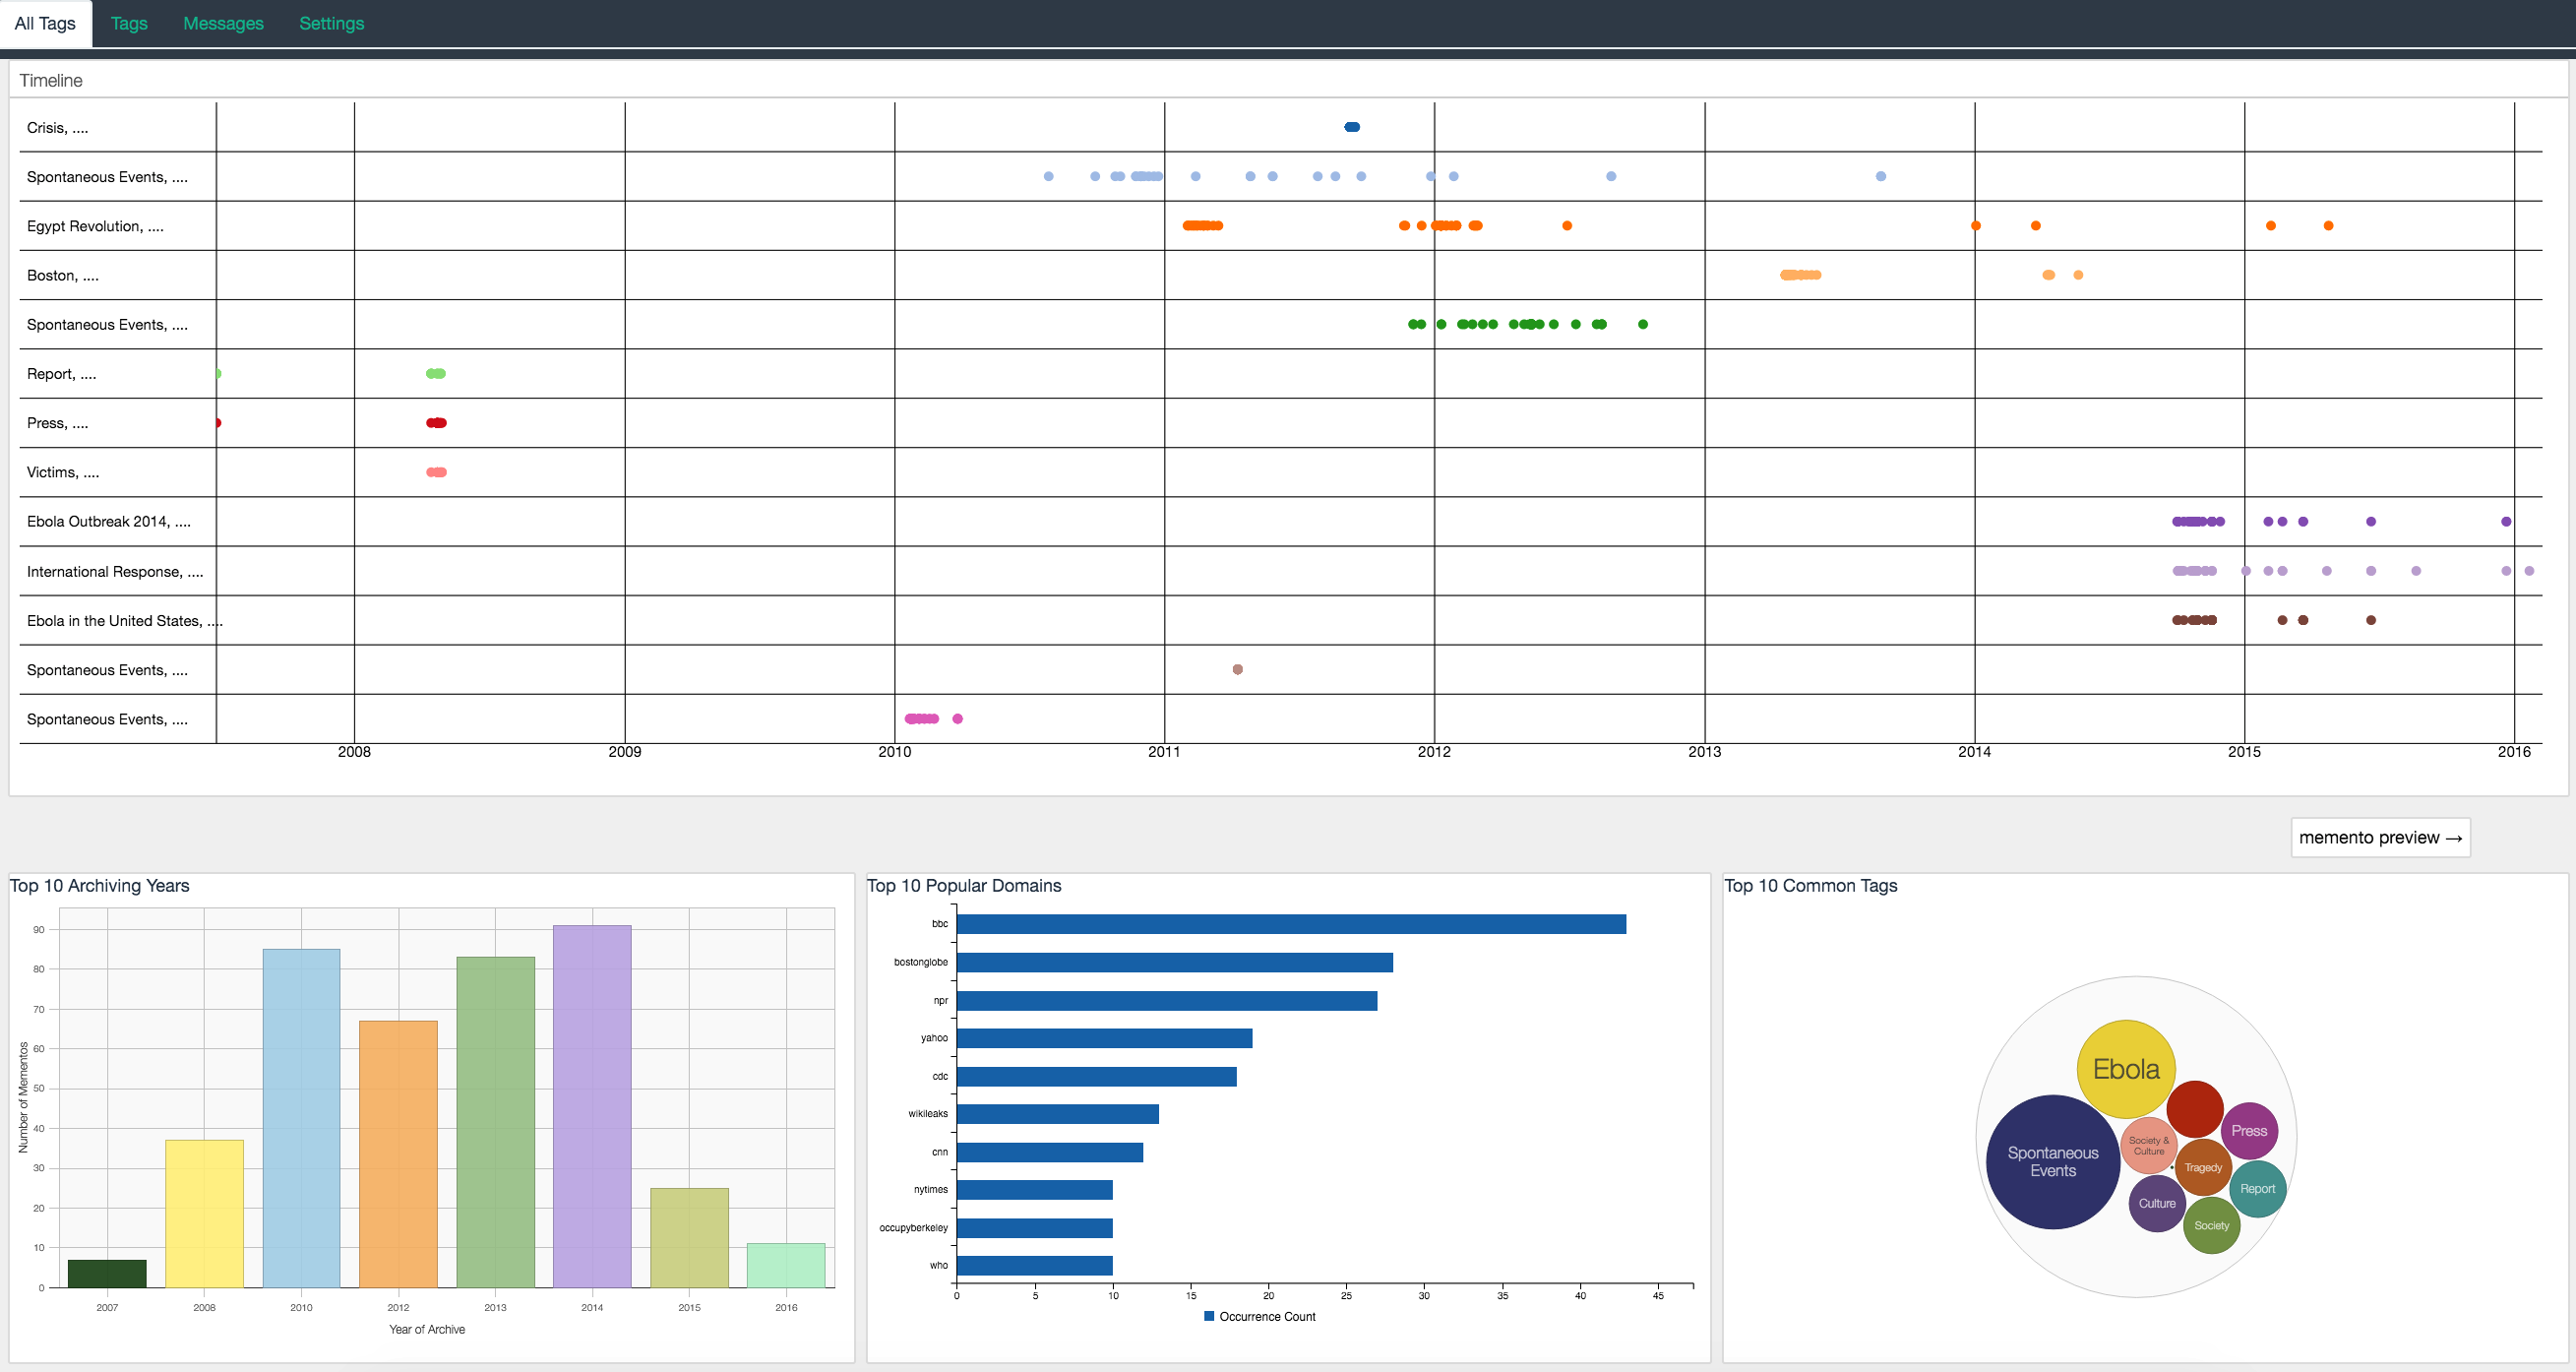
\includegraphics[scale=0.1]{Figure1}
\caption{Web Archive Visualizer}
\label{fig:mesh1}
\end{figure} 

In our current solution, Web Archive Visualizer, we propose an approach that addresses those problems. The idea behind our solution is that contextual information created during time of archive, such as the name and keywords associated with a resource, can create a set of useful characteristics about the data. Using this additional information, we are not only able to relate sub sections of an archive, but also limit both the amount and the types of resources shown. While the cost of going through the archival process is noticeably higher, the potential increase in overall understanding far outweighs its limitations. Web Archive Visualizer can be seen in Fig. 1, where the system is separated into multiple views denoting particular points of interest. \par

\begin{figure*}
\centering
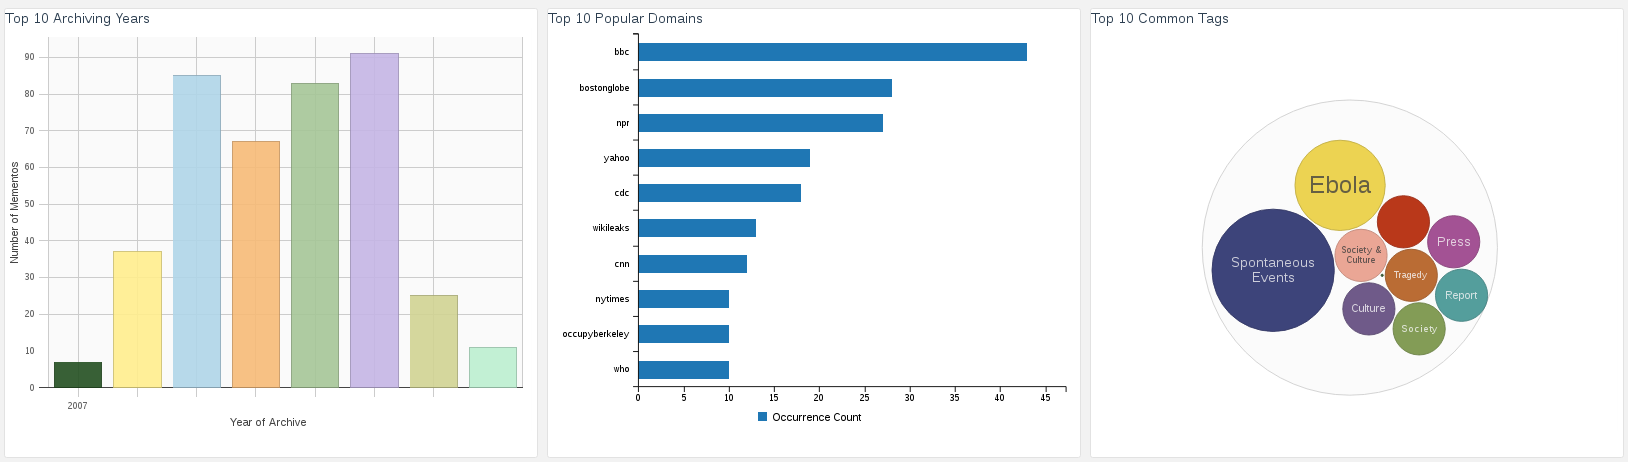
\includegraphics[width=\textwidth]{Figure3a}
\caption{This figure shows the general idioms that apply to the entire collection.}
\label{fig:mesh2}
\end{figure*}

\section{Related Work}
The vast majority of current and previous works of web archive visualizations places a heavy focus on their evolution. Dating back to 2005, the developers behind WebRelievo \cite{toyoda2005system} propose a visualization to monitor the change of resources within a web archive over a particular period. Aside from a known archival date, the goal of the system aims to identify relationships between different web resources without any contextual data. In another words, they aim to see the interconnecting of the web and how it differs over a span of years, without taking any additional characteristics from the original archivers. Even though there is a lack of contextual data, WebRelievo proposes a good step towards relationship identification of resources within collections, regardless of the collection size. \par

Older works, such as those in \cite{toyoda2003extracting}, show relationships between resources located within similar communities. In this context, communities are clusters that all relate to a particular topic. While this approach also uses only temporal attributes of the archival process, the authors show the importance of identifying points of interest within a web archive. The general idea of this work directly supports ours, in which we leverage relationship identification of like meta data, i.e. tags and temporal attributes, to help classify and discover potential areas of interest. \par


\section{Design}
The real estate of the viewers attention is split into multiple views of interest, as seen in Figure \ref{fig:mesh1}. In both the top and bottom portion of the screen, referred to as the main content, users are given the ability to view specific characteristics of all data within the archive. The main content is complemented with arrows to help navigate between different specific views. In addition, text of the navigation links dynamically changes to alert the user about the next and previous idioms in line. We find this a helpful feature, where the element of surprise is limited, allowing the user to anticipate and possibly expand their exploration towards more specific charts.  \par

On the contrary, the middle portion outlines multiple views for more general characteristics that can summarize the entire collection. We refer to this section as the complementary content. Note, the split of interest between these two sections is important, as it gives users more control on the amount of data that they see at once. In essence, this is a strategically enforced measure to ensure cognitive memory does not become overloaded. Unlike the main content, views within the complementary content are always shown. The proactive enforcement of this idiom enables comparison between the more specific and summarized contents shown within the web archive collection. Its centered location on the screen complements this use as it stays within the real estate bounds of different views. \par

To make the boundary between main and complementary contents more clear to the user, we separate generated visualizations by the area of categorical influence. This causes resource specific views to fall into several categories, including: timeline of resource archives, thumbnail views of mementos, resource clusters, and keyword groupings. They are granular enough to ensure that the targeted audience can fork out and create relationships of the low level details surrounding their data. On the contrary, idioms showing general characteristics primarily focus on the higher level summaries, such as outlining the most active archiving years, popular domains, and the most common tags. \par 

\begin{figure*}
\centering
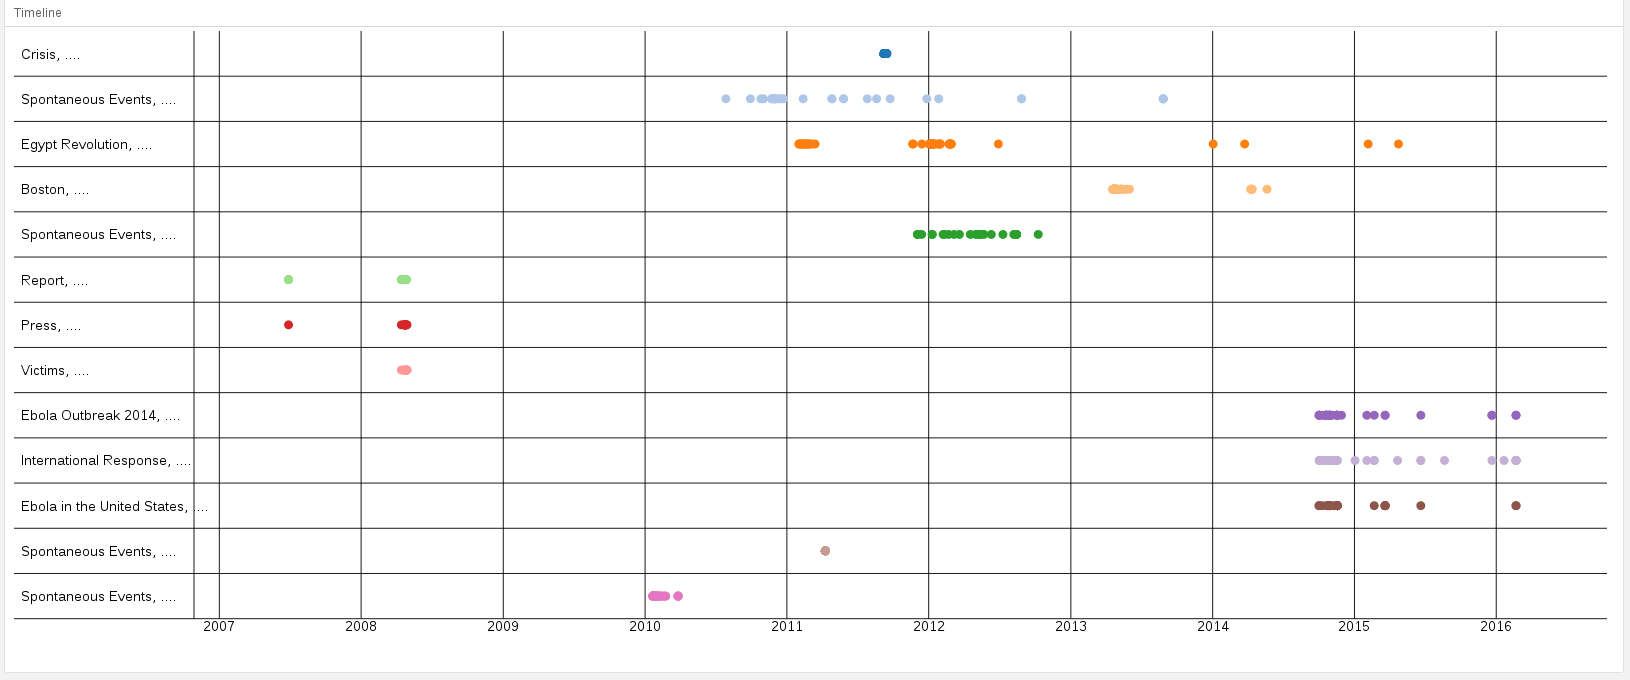
\includegraphics[width=\textwidth]{Figure4}
\caption{Timespan chart showing archives associated with particular tags}
\label{fig:mesh3}
\end{figure*}

\subsection{Resource specific idioms}
One of the primary areas of focus, alike most recent work, is time. Knowing when a particular resource was archived, is the first step in identifying differences over a lifetime and drawing conclusions as to how temporal periods affected particular resources. For this reason, Web Archive Visualizer places primary focus on the Timeline view, as seen in Figure \ref{fig:mesh3}. The purpose of this idiom is to let users view keywords associated with archived resources, over time. Aside from the obvious, keyword dominance over time, this chart also allows us to see the levels of activity as the collection years grow. When zoomed out, the scatterplot can outline this trend easily, leading us towards identifying temporal trends and outliers within our collection. \par

Another resource specific idiom presented in our vis is wordplay, as shown in figure \ref{fig:mesh6}. The purpose of this idiom is to outline the keyword clusters and its associations between resources and mementos. Its use is primarily evident when one wants to identify areas that are created by different keywords. Take for example a keyword ``cat''. By using this view, the user can see mementos and resources that are centered around ``cats''. In addition, the view allows us to create a cluster of like words, that are also found within points of interest. In the above example, this would create a closer distance between keywords like ``animals'' and ``cats''. Lastly, if the categorical number of keywords becomes exponentially difficult to manage due to its size, filtering and zooming will create a controlled setting for many prospective users. \par

Web Archive Visualizer also contains a keyword bar chart, which allows users to view the associated counts of different tags, and how they relate to the rest of the collection. Depending on the area of focus in the archive, this particular idiom can be a great identifier of primary word associations in the archiving efforts. It can help answer questions such as: ``What words are primarily found in the web archives?'' and ``Is there a shift in categories of those words within the entire collection, or do they all fall within a similar scope?'' \par 

For those who find bar chart counts limiting, the system also provides temporal tree maps. This idiom takes the bar chart results a bit further, in which they identify the spread of keywords over time for both resources and mementos. While a bar chart showing keyword counts can help answer many questions, temporal tree maps can provide reasoning and awareness as to why those counts have their respectful values. This idiom allows for navigation through the years, and resources, allowing the user to pinpoint exactly what time is primarily responsible for an increase or decrease in keyword associations. Temporal tree maps also have another large benefit, in which they present size with importance per year. This makes it especially easy to compare how particular keywords relate to the remainder of the collection within a year. \par

Lastly, the system concludes resource specific views with the inclusion of keyword timegraphs, and their association with resources and mementos. This idiom aims to show both overlaps in archiving and which domains are responsible for the basis of our entire collection. Note, while there is no single correct chart to use when answering a diverse amount of questions, it is the goal of these specific views to help answer as many as possible by emphasizing their collaborative use. In some cases, many views can answer several different questions, but the ease of getting that answer will drastically differ between the idioms of choice. \par

\subsection{General idioms}
Figure \ref{fig:mesh2} shows three different general views. The left most view, memento activity over a set of years, denotes the number of archives present for a particular resource in some time. Understanding the most active years has many advantages to archivers and general users exploring the collection. First, it allows them to conceptually visualize what periods of activity are responsible for the peaks within the collection. If the collection has a specific context, such as an archive consisting of hurricane events, particular years could outline the most influential years. The same is also true for identifying trends or outliers in data, where particular years might show a steady incline, decline, or abnormal levels of mementos collected. \par

Most popular domains, middle view in Figure \ref{fig:mesh2}, shows where most of the resources are being collected from. This is especially important to know when understanding domain reliance or influence of content of the web archive. Alike the idiom denoting years, understanding domain dominance can also help outline the skewness and bias within our collections. This is especially helpful, when the archiving team is collecting mementos relating to one particular category from a limitless scope of domains. \par

The last view in Figure \ref{fig:mesh2} shows the most popular tags, whose occurrence count is represented in an increased size. Once a tag dominates others, we can gain more contextual awareness regarding our data. This can help us answer questions like: "Are we focusing on archiving particular areas?" and "Are there particular keywords associated with our collection subset?". Having this general view is also especially helpful when attempting to compare results found in the views of main content. By having two different keywords for comparison, we can begin to see dominance between the words of interest and those that are most popular. \par

\begin{figure*}
\centering
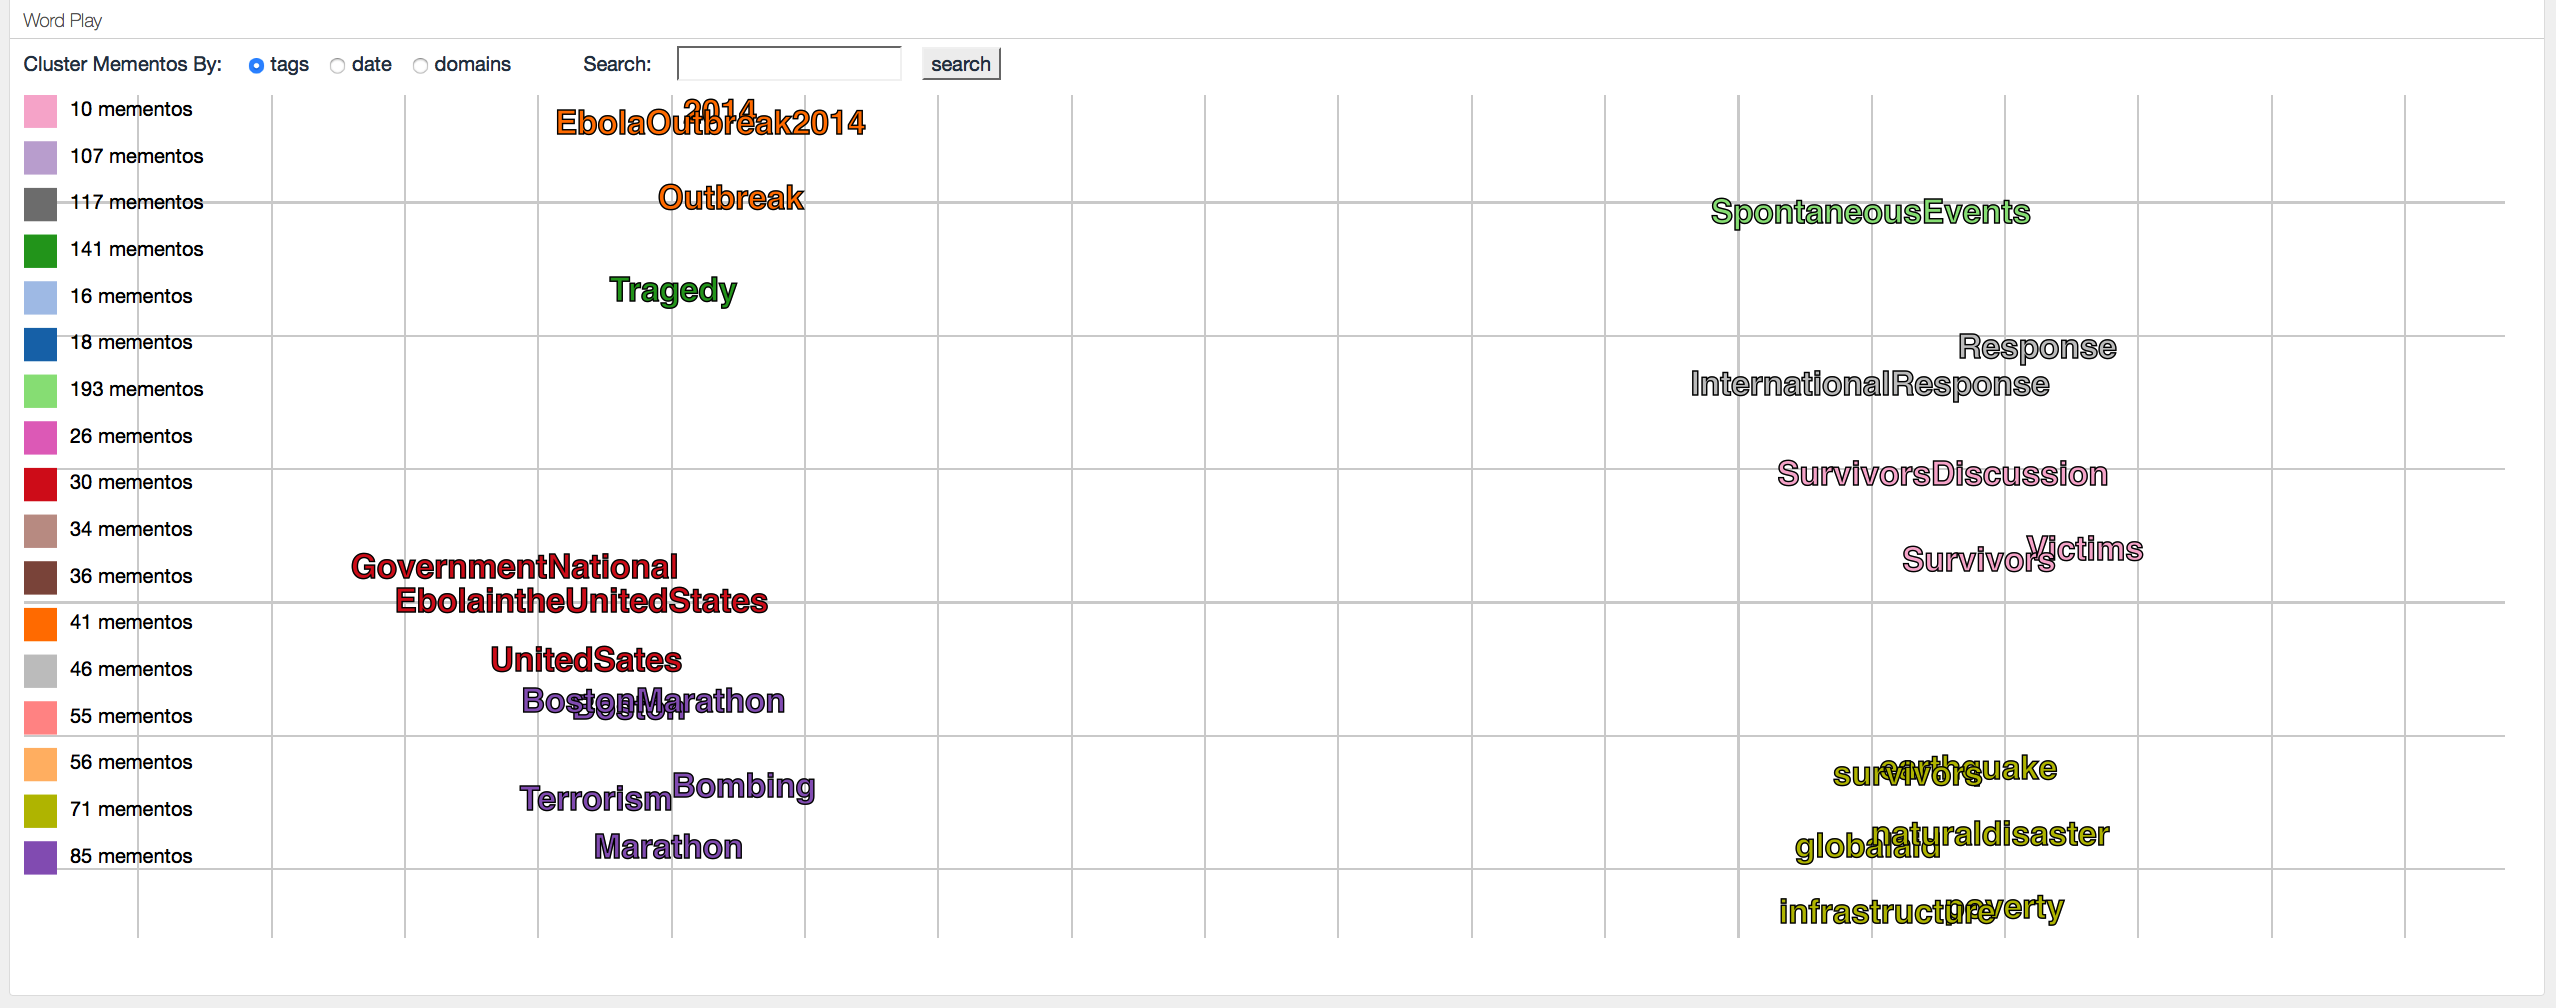
\includegraphics[width=\textwidth]{Figure6}
\caption{Word play showing clusters and tag associations}
\label{fig:mesh6}
\end{figure*}


\subsection{What Why How Framework}
Web Archive Visualizer was created as part of the Information Visualization class taught
at Old Dominion University. In it we read through Tamara Munzner's "Visualization 
Analysis and Design", in which she presents a framework for the systematic analysis
of visualizations and a common language for their evaluation; the What, Why, How 
Framework. The What, Why, How Framework provides abstractions for validating visualizations
at four distinct, nested levels of design. These are the Domain, Data/Task Abstraction, Encoding/Interaction Idiom, and Algorithm levels.
This project's scope and duration did not allow explicitly performing the different
validation techniques discussed by Munzner at the different levels. 
However, we justify the decisions made at each level with respect to the What, Why, How 
Framework next.

Our domain situation is explicitly characterized by the work and research performed by web archivers. 
Web archivers digitally preserve records so that we can later replay and study them. 
In the course of doing so, they amass collections which they need to share and 
query for facts in general. These problems of search, analysis, and query directly 
benefit from our vis tool support. 

At the domain situation level we characterize URI-M collections from the digital preservation domain.
A collection of mementos includes URI-Ms associated to different attributes such as tags, dates, archiver, 
and URI-R. We then produced a design that comes from requirements formalized by several interviews performed 
with the course instructor.

At the data/task abstraction level we represent the collection of URI-Ms as a table
with a number of items made up of a number of attributes. We did this to facilitate 
identifying a varied number of abstract tasks. Tables can be easily sorted and aggregated
enabling a number of actions and targets. Attributes can also be easily appended or removed
from a table without necessarily altering the views that present the data.

One of our primary goals of the developed system was supporting a wide number of abstract tasks. Because of this
we produced a system with a number of varied views, each supporting a unique set of
actions and targets.

We support the discover action via views that provide knowledge that was not previously known.
Complementary views, top 10 charts addressing different areas, are examples of this. We support the present action via a number of timelines 
which can be used for expressing how the data evolves over time. 
We also support general enjoyment; our visualization makes it much easier to digest the
collection overall in comparison to its spreadsheet form. We support the 
lookup action via our word map view in which a specific (or incomplete) item or 
attribute can search for (or looked up), and then explored as a table for a number of individual
targets. Our treemap, view supports the browse and explore action, allowing the dynamic 
navigation of item sets aggregated by different attributes. Finally, our visualization allows 
compare and summarize via our juxtaposed complementary views. Most of our abstract targets
involve individual items, individual attributes, and trends over time.

At the encoding/interaction level we made three primary decisions. The first is 
more of a rule of thumb, rather than an explicit encoding. It is the rule of thumb 
discussed by Munzner as "Overview First, Zoom and Filter, Details on Demand". 
A large chunk of our screen real estate is dedicated to summarize oriented idioms. 
These idioms start the user off with a general awareness of the entire information space
and allow requesting incrementally specific item subsets categorized by multiple attributes.

The second decision was the inclusion and utilization of juxtaposed views.
Given a varied number of abstract tasks, we felt that the overall delivery efficiency would
be maximized by juxtaposing a number of smaller navigable views, each subject to its
own secondary encodings. Some of these include ordering, selection, navigation, and
the encoding of different attributes via color hue.

The third decision centered around extensive use of filtering and aggregation. A consistently driving goal 
was providing access to a dataset that lacks semantics in its raw form. Many of our
individual views aggregate data items by attribute and filter for items of interest 
in attempts to mitigate cognitive load on the user. 

All in all, the primary goal of this visualization system was to provide access to an otherwise inaccessible dataset.
Via the use of multiple idioms (summarized above) we present the dataset
from multiple, varied perspectives that enable effective analysis, search, and query.

\begin{table}
\renewcommand{\arraystretch}{1.3}
\caption{What Why How Framework}
\label{tab:example}
\centering
\begin{tabular}{l|l}
    \hline
    Idiom  &  Web Archive Visualizer\\
    \hline
    \hline
	What: Data & Web archive collection \\ \hline
	What: Derived & Table with multiple attributes \\   \hline
	Why: Tasks & \parbox[t]{5cm}{Discover trends over time, discover extremes, general enjoyment, lookup, browse, locate, and explore individual items and items grouped by attribute, identify individual items, compare and summarize data} \\ \hline
	How: Encode & \parbox[t]{5cm}{Timeline,  Time Graph, Bar Chart, Histogram, Bubble Chart, Word Map, Treemap} \\ \hline
	How: Manipulate & Navigate, Pan, Zoom \\  \hline
	How: Facet & Juxtapose views \\  \hline
	How: Arrange & Separate, Order, Align \\ \hline
	How: Map & Size and area for quantity, color hue for category \\ \hline
	How: Reduce & Aggregation and filtering \\  \hline
Scale & \parbox[t]{5cm}{Attributes: half a dozen, Total items: several hundred} \\
	\\
    \hline
\end{tabular}
\end{table}

\section{Performance Testing}

To perform performance testing, we ran an analysis for load times of our visualization. The system used for experimentation comprises of the following hardware: AMD A6-3650 Llano Quad-Core 2.6 CPU, 4GB of RAM, and a 5400RPM 100GB hard drive. It is running Windows 7 and Google Chrome Version 50.0.2661.86 (64-bit). \par

\begin{figure}[b]
\centering
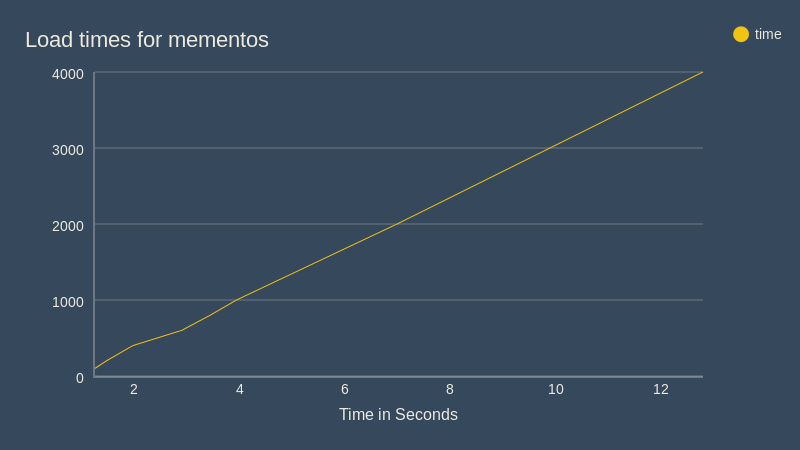
\includegraphics[scale=0.3]{Figure5}
\caption{Duration of loading mementos over time}
\label{fig:mesh4}
\end{figure}

Looking at Figure \ref{fig:mesh4}, we are able to conclude that the performance of the Web Archive Visualizer is able to handle several hundred mementos. The system becomes much more strained as the memento counts get into several thousands. In respect to our goal, several hundred resources are the aim of moderately sized collection, whose times of loading fall within 2 seconds. For large collections, which were out of our scope, there is an exponential trend in load times. \par

\section{Conclusion}
Understanding and creating relationships within web archives are tasks that can quickly become difficult to manage. When the size of the collection is relatively small, those tasks can usually be easy to accomplish. However, as the collection grows into several hundred results, the difficulty of completing our tasks becomes much more difficult. For this, we propose a new system towards understanding moderately sized collections called the Web Archive Visualizer. Using contextual data provided during the archive process, such as keywords and temporal attributes, the proposed system outlines and answers questions about a collection that can be helpful to a wide variety of audiences. Novice users looking to explore data and researchers discovering particular trends, can both utilize the developed system for their intended task. \par

Web archive Visualizer is able to accomplish its goals by creating resource specific and general views. This split of information is a strategic approach to conserving cognitive memory, while allowing attention and focus towards particular areas of interest. The specific views allow for more low level characteristic analysis, spanning results in the entire collection. This includes idioms such as: bar chart showing counts of all keywords, timespan analysis of mementos, and the temporal evolution of resource archives. On the other hand, general views give us a higher level analysis of our collection, in which they summarize our collection. Having a combination of both is crucial, as the number of possible answers and comparison analytics can promote a larger understanding for our audience. \par

\section{Final Thoughts}
Looking towards the future, it is clear that our current system would significantly benefit from the use of contextual linking and highlighting. While the views presented in the Web Archive Visualizer have their primary intentions of use, synchronizing areas of focus across all views would significantly improve user experience. It is our belief that aside from easier navigation, the intended audience would be able to perform comparisons and attribute localization both quicker and easier. \par

In the context of future evaluation, we aim to perform validation analysis on the system. We could use this analysis to improve, or reshape, the views that the users are looking to see and actually have. In addition, as more like tools arise, tests can be performed to identify which tools are the most useful in understanding moderately sized collections, and how our designed system compares to them. \par


% Can use something like this to put references on a page
% by themselves when using endfloat and the captionsoff option.
\ifCLASSOPTIONcaptionsoff
  \newpage
\fi



% trigger a \newpage just before the given reference
% number - used to balance the columns on the last page
% adjust value as needed - may need to be readjusted if
% the document is modified later
%\IEEEtriggeratref{8}
% The "triggered" command can be changed if desired:
%\IEEEtriggercmd{\enlargethispage{-5in}}

% references section
\bibliography{mybib}{}

% can use a bibliography generated by BibTeX as a .bbl file
% BibTeX documentation can be easily obtained at:
% http://mirror.ctan.org/biblio/bibtex/contrib/doc/
% The IEEEtran BibTeX style support page is at:
% http://www.michaelshell.org/tex/ieeetran/bibtex/
\bibliographystyle{IEEEtran}
% argument is your BibTeX string definitions and bibliography database(s)
%\bibliography{IEEEabrv,../bib/paper}
%
% <OR> manually copy in the resultant .bbl file
% set second argument of \begin to the number of references
% (used to reserve space for the reference number labels box)

\end{document}


